\scanpage{62}
\begin{center}
U N I V E R S I T E\\
DES SCIENCES ET TECHNIQUES\\
DU LANGUEDOC\\
-{}-{}-{}-{}-{}-{}-{}-{}-{}-{}-{}-\\
Service de la Scolarité\\
MR / GJ\\
Diffusion : Liste A\\
N\textdegree\ : 4151
\end{center}
Montpellier, le 1er Juillet 1978

\begin{center}
\uline{AVIS DE SOUTENANCE D'UNE THESE DE DOCTORAT DE 3ème CYCLE}

\uline{(PHYSIQUE DU SOLIDE - APPLICATION A L'ELECTRONIQUE )}
\end{center}

\uline{Nom et prénom de la candidate} : MERLET née BERNARD Catherine

\uline{Titre de la thèse} : Le phénomène de gel magnétique dans InSb : étude en fonction
du dopage.

\uline{Date, heure et lieu de soutenance prévus} :

12 JUILLET 1978 à 15 Heures,

Salle de Séminaire du C.E.E.S.- U.S.T.L.

\uline{Nom du Directeur de thèse} :

Monsieur le Professeur ROBERT.

\uline{Désignation du laboratoire où la thèse est préparée} :

Centre d'Etudes d'Electronique des Solides, MONTPELLIER.

\uline{Analyse de l'ouvrage} :

L'étude du phénomène de gel magnétique a été
faite sur des échantillons d'InSb différemment dopés (\(10^{14}\)à \(10^{16}\mathrm{cm}^{-3}\)). Ce
phénomène se traduit par une variation de l'énergie de liaison en fonction du
dopage. Pour les échantillons faiblement dopés on a mis en évidence la localisa-\\
tion d'une partie des porteurs de la bande de conduction à faible température.

\uline{Durée approximative des recherches ayant abouti à la thèse} : Deux ans

\uline{Composition du jury proposé} :

\diagram{\(\begin{array}{lll}
\text{MM.}&:&\\
&&\text{PISTOULET, Président}\\
&&\text{ROBERT}\\
&&\text{RAYMOND}\\
&&\text{LEROUX HUGON}\\
&&\text{THUILLIER}
\end{array}\)}

Le Secrétaire Général,

\figure{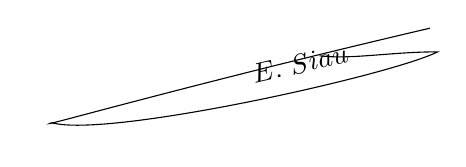
\begin{tikzpicture}
\draw (-2.7,-0.7) .. controls (-3,-0.8) and (-0.9,-0.2) .. (2.1,0.5);
\draw (-2.7,-0.7) .. controls (-2,-0.9) and (1.6,-0.1) .. (2.2,0.2)
.. controls (1.6,0.2) and (1.1,0.1) .. (0.7,0.15);
\node[rotate=13] at (0.45,0.05) {\(\unsure{E.\ Siau}\)};
\end{tikzpicture}}

\uline{E. SIAU}
\mspage{61}

